\documentclass[a4paper, 14pt]{article}
\usepackage[T2A]{fontenc}
\usepackage[utf8]{inputenc}
\usepackage[english,russian]{babel}
\usepackage[left = 3cm, right = 2cm, top = 2cm, bottom = 2 cm]{geometry}
\usepackage{graphicx}
\usepackage{listings}
\usepackage{color}
\usepackage{amsmath}
\usepackage{pgfplots}
\usepackage{url}
\usepackage{tikz}
\usepackage{float}
\usepackage{multirow}

\usepackage{titlesec}
\titleformat*{\section}{\LARGE\bfseries}
\titleformat*{\subsection}{\Large\bfseries}
\titleformat*{\subsubsection}{\large\bfseries}
\titleformat*{\paragraph}{\large\bfseries}
\titleformat*{\subparagraph}{\large\bfseries}

\lstset{
	language=Python, 
	numbers=left,   
	frame=single, 
	escapebegin=\begin{russian}\commentfont,
    escapeend=\end{russian},
    breaklines=true,   
    breakatwhitespace=true,
	literate={а}{{\selectfont\char224}}1
	{б}{{\selectfont\char225}}1
	{в}{{\selectfont\char226}}1
	{г}{{\selectfont\char227}}1
	{д}{{\selectfont\char228}}1
	{е}{{\selectfont\char229}}1
	{ё}{{\"e}}1
	{ж}{{\selectfont\char230}}1
	{з}{{\selectfont\char231}}1
	{и}{{\selectfont\char232}}1
	{й}{{\selectfont\char233}}1
	{к}{{\selectfont\char234}}1
	{л}{{\selectfont\char235}}1
	{м}{{\selectfont\char236}}1
	{н}{{\selectfont\char237}}1
	{о}{{\selectfont\char238}}1
	{п}{{\selectfont\char239}}1
	{р}{{\selectfont\char240}}1
	{с}{{\selectfont\char241}}1
	{т}{{\selectfont\char242}}1
	{у}{{\selectfont\char243}}1
	{ф}{{\selectfont\char244}}1
	{х}{{\selectfont\char245}}1
	{ц}{{\selectfont\char246}}1
	{ч}{{\selectfont\char247}}1
	{ш}{{\selectfont\char248}}1
	{щ}{{\selectfont\char249}}1
	{ъ}{{\selectfont\char250}}1
	{ы}{{\selectfont\char251}}1
	{ь}{{\selectfont\char252}}1
	{э}{{\selectfont\char253}}1
	{ю}{{\selectfont\char254}}1
	{я}{{\selectfont\char255}}1
	{А}{{\selectfont\char192}}1
	{Б}{{\selectfont\char193}}1
	{В}{{\selectfont\char194}}1
	{Г}{{\selectfont\char195}}1
	{Д}{{\selectfont\char196}}1
	{Е}{{\selectfont\char197}}1
	{Ё}{{\"E}}1
	{Ж}{{\selectfont\char198}}1
	{З}{{\selectfont\char199}}1
	{И}{{\selectfont\char200}}1
	{Й}{{\selectfont\char201}}1
	{К}{{\selectfont\char202}}1
	{Л}{{\selectfont\char203}}1
	{М}{{\selectfont\char204}}1
	{Н}{{\selectfont\char205}}1
	{О}{{\selectfont\char206}}1
	{П}{{\selectfont\char207}}1
	{Р}{{\selectfont\char208}}1
	{С}{{\selectfont\char209}}1
	{Т}{{\selectfont\char210}}1
	{У}{{\selectfont\char211}}1
	{Ф}{{\selectfont\char212}}1
	{Х}{{\selectfont\char213}}1
	{Ц}{{\selectfont\char214}}1
	{Ч}{{\selectfont\char215}}1
	{Ш}{{\selectfont\char216}}1
	{Щ}{{\selectfont\char217}}1
	{Ъ}{{\selectfont\char218}}1
	{Ы}{{\selectfont\char219}}1
	{Ь}{{\selectfont\char220}}1
	{Э}{{\selectfont\char221}}1
	{Ю}{{\selectfont\char222}}1
	{Я}{{\selectfont\char223}}1
}

\newcommand{\biglisting}[1]{%
	\lstinputlisting[numbers=left]{#1}%
}

\begin{document}

	\textbf{Цель работы:} получение навыков разработки  алгоритмов решения краевой задачи при реализации моделей, построенных на  ОДУ второго порядка.\\
	
	
	\section{Теоретическая часть}
	
Задана математическая модель.\\
Уравнение для функции  $T(x)$:\\
\begin{equation}
\frac{d}{dx}\bigg(K(x)\frac{dT}{dx}\bigg)-\frac{2}{R}\alpha(x)T+\frac{2T_0}{R}\alpha(x)=0
\end{equation}

Краевые условия:\\
\begin{equation}
 \begin{cases}
   x=0, ~-k(0)\frac{dT}{dx}=F_0
   \\
   x =l,~-k(l)\frac{dT}{dx}=\alpha_N(T(l)-T_0)
 \end{cases}
\end{equation}
 
 Функции $k(x), \alpha(x)$ заданы:
\begin{equation}
k(x)=\frac{a}{x-b}
\end{equation}
\begin{equation}
\alpha(x)=\frac{c}{x-d}
\end{equation}

Константы $a, b$  следует найти из условий $k(0) = k_0, k(l) = k_N$, а константы  $c, d$ из условий  $\alpha(0) = \alpha_0, \alpha(l)=\alpha_N$.

\begin{equation}
a = -k_0b
\end{equation}
\begin{equation}
b = \frac{k_Nl}{k_N-k_0}
\end{equation}
\begin{equation}
c = -\alpha_0d
\end{equation}
\begin{equation}
d = \frac{\alpha_0l}{\alpha_N-\alpha_0}
\end{equation}
 
 Разностная схема

\begin{equation}
\begin{aligned}
&A_ny_{n-1}-B_ny_n+C_ny_{n+1}=-D_n, 1\le n\le N-1\\
&K_0y_0+M_0y_1=P_0\\
&K_Ny_N+M_Ny_{N-1}=P_N
\end{aligned}
\end{equation}
, где

\begin{equation}
A_n=\frac{x_{n+\frac{1}{2}}}{h},
\end{equation}
\begin{equation}
B_n=A_n+C_n+p_nh,
\end{equation}
\begin{equation}
C_n=\frac{x_{n-\frac{1}{2}}}{h},
\end{equation}
\begin{equation}
D_n=f_nh
\end{equation}

Для вычисления используем метод средних:
\begin{equation}
x_{n\pm\frac{1}{2}}=\frac{k_n+k_{n\pm1}}{2}
\end{equation}

Система решается в два прохода: прямой и обратный.

В прямом проходе вычисляем прогоночные коэффициенты $\varepsilon$ и $\eta$. Начальные значения:

\begin{equation}
\begin{aligned}
&\varepsilon_1=-\frac{M_0}{K_0}\\
&\eta_1=\frac{P_0}{K_0}
\end{aligned}
\end{equation}
\newpage
Вычисляем массивы прогоночных коэффициентов $\varepsilon, \eta$:

\begin{equation}
\begin{aligned}
&\varepsilon_{n+1} = \frac{C_n}{B_n-A_n\varepsilon_n}\\
&\eta_{n+1} = \frac{D_n+A_n\eta_n}{B_n-A_n\varepsilon_n}
\end{aligned}
\end{equation}

Обратный проход.

Определим $y_N$ - значение функции в последней точке:

\begin{equation}
y_N=\frac{P_N-M_N\eta_N}{K_N+M_N\varepsilon_N}
\end{equation}

По основной прогоночной формуле находятся все значения неизвестных $y_n$:
\begin{equation}
y_n=\varepsilon_{n+1}y_{n+1}+\eta_{n+1}
\end{equation}

Таким образом, массив, полученный после прогонки и есть искомый массив T(x). \\

\subsection*{Краевые условия}
Обозначим:
\begin{equation}
\begin{aligned}
&F=-k(x)\frac{dT}{dx}\\
&p(x)=\frac{2}{R}\alpha(x)\\
&f(x)=\frac{2T_0}{R}\alpha(x)\\
&p_n=p(x_n), ~f_n=f(x_n)
\end{aligned}
\end{equation}

Разностные аналоги краевых условий при $x=0$ (из лекции № 7):

\begin{equation}
\bigg(x_{\frac{1}{2}} + \frac{h^2}{8}p_{\frac{1}{2}}+\frac{h^2}{4}p_0\bigg) \cdot y_0 - \bigg(x_{\frac{1}{2}}-\frac{h^2}{8}p_{\frac{1}{2}}\bigg) \cdot y_1=\bigg(hF_0+\frac{h^2}{4}(f_{\frac{1}{2}}+f_0)\bigg)
\end{equation}

Разностные аналоги краевых условий при $x=l$:\\

Примем простую аппроксимацию:
\begin{equation}
\begin{aligned}
&p_{\frac{1}{2}}=\frac{p_0+p_1}{2}\\
&f_{\frac{1}{2}}=\frac{f_0+f_1}{2}\
\end{aligned}
\end{equation}

Проинтегрируем уравнение (1) на отрезке $[x_{N-\frac{1}{2}}, x_N]$ с учетом замен (19).

$$-\int^{X_N}_{X_{N-{\frac{1}{2}}}}\frac{dF}{dx}dx-\int^{X_N}_{X_{N-{\frac{1}{2}}}}p(x)Tdx+\int^{X_N}_{X_{N-{\frac{1}{2}}}}f(x)dx=0$$

Второй и третий интегралы вычислим методом трапеций

$$F_{N-\frac{1}{2}}-F_N-\frac{p_{N-\frac{1}{2}}y_{N-\frac{1}{2}}+p_Ny_N}{4}h+\frac{f_{N-\frac{1}{2}}+f_N}{4}h=0$$

Учтем, что

$$F_{N-\frac{1}{2}}=x_{N-\frac{1}{2}}\frac{y_{N-1}-y_N}{h}$$
$$F_N=\alpha_N(y_N-T_0)$$
$$y_{N-\frac{1}{2}}=\frac{y_N+y_{N-1}}{2}$$

После подстановки и приведения подобных получаем:

\begin{equation}
\bigg(-\frac{x_{N-\frac{1}{2}}}{h} - \alpha_N - \frac{2p_N - 1}{16}h\bigg) \cdot y_N + \bigg (\frac{x_{N-\frac{1}{2}}}{h} - \frac{2p_N - 1}{16}h\bigg) \cdot y_{N-1} = - \alpha_NT_0 - \frac{h}{4} \bigg({f_{N-\frac{1}{2}}+f_N}\bigg)
\end{equation} 

Заданы начальные параметры:\\ \\
$k_0$ = 0.4 Вт/см К,\\
$k_N$ = 0.1 Вт/см К,\\
$\alpha_0$ =  0.05 Вт/см2 К,\\
$\alpha_N$ = 0.01 Вт/см2 К,\\
$l$ =  10 см,\\
$T_0$ =  300К,\\
$R$ =  0.5 см,\\
$F_0$ =  50 Вт/см2.


\subsection*{Физическое содержание задачи}

Сформулированная математическая модель описывает температурное поле $T(x)$ вдоль  цилиндрического стержня радиуса $R$ и длиной  $l$ , причем $R<<l$  и температуру можно принять постоянной по радиусу цилиндра. Ось $x$ направлена вдоль оси цилиндра и начало координат совпадает с левым торцем стержня. Слева при $x=0$ цилиндр нагружается тепловым потоком  . Стержень обдувается воздухом, температура которого равна $T_0$ . В результате происходит съем тепла с цилиндрической поверхности и поверхности правого торца при  $x=l$. Функции $k(x), \alpha(x)$ являются, соответственно, коэффициентами теплопроводности материала стержня и теплоотдачи при обдуве,.

\section{Практическая часть}

В листинге 1 представлен код программы:

	\begin{lstlisting}[label=some-code,caption=Листинг программы]
import matplotlib.pyplot as plt
import numpy as np

# коэффициенты теплопроводности и теплоотдачи
def k(x):
    return a / (x - b)

def alpha(x):
    return c / (x - d)


def p(x):
    return 2 * alpha(x) / R

def f(x):
    return 2 * alpha(x) * T0 / R


# метод средних
def x_plus_half(x):
    return (k(x) + k(x + h)) / 2

def x_minus_half(x):
    return (k(x) + k(x - h)) / 2
    

# коэффициенты разностной схемы
def A(x):
    return x_plus_half(x) / h

def C(x):
    return x_minus_half(x) / h

def B(x):
    return A(x) + C(x) + p(x) * h

def D(x):
    return f(x) * h


# левое граничное условие
def left_boundary_condition():
    K0 = x_plus_half(0) + h * h * (p(0) + p(h)) / 16 + h * h * p(0) / 4
    M0 = -x_plus_half(0) + h * h * (p(0) + p(h)) / 16
    P0 = h * F0 + h * h / 4 * ((f(0) + f(h)) / 2 + f(0))
    return K0, M0, P0

# правое граничное условие
def right_boundary_condition():
    KN = -x_minus_half(l) / h - aN - p(l) * h / 4 - ((p(l) + p(l - h)) * h) / 16
    MN = x_minus_half(l) / h - ((p(l) + p(l - h)) * h) / 16
    PN = - aN * T0  -  h * (f(l) + f(l - h) + f(l)) / 8
    return KN, MN, PN


if __name__ == "__main__":
    K0 = 0.4
    KN = 0.1
    a0 = 0.05
    aN = 0.01
    l = 10
    T0 = 300
    R = 0.5
    F0 = 0
    h = 1e-3

    # параметры коэффициентов теплопроводности и теплоотдачи
    b = (KN * l) / (KN - K0)
    a = - K0 * b
    d = (aN * l) / (aN - a0)
    c = - a0 * d

    K0, M0, P0 = left_boundary_condition()
    KN, MN, PN = right_boundary_condition()

    # прямой ход
    # массивы прогоночных коэффициентов
    eps = [0]
    eta = [0]

    eps1 = -M0 / K0
    eta1 = P0 / K0

    eps.append(eps1)
    eta.append(eta1)

    x = h
    n = 1
    while x + h < l:
        eps.append(C(x) / (B(x) - A(x) * eps[n]))
        eta.append((A(x) * eta[n] + D(x)) / (B(x) - A(x) * eps[n]))
        n += 1
        x += h

    # обратный ход
    t = [0] * (n + 1)
    # значение функции в последней точке
    t[n] = (PN - MN * eta[n]) / (KN + MN * eps[n])

    for i in range(n - 1, -1, -1):
        t[i] = eps[i + 1] * t[i + 1] + eta[i + 1]

    x = [i for i in np.arange(0, l, h)]

    plt.plot(x, t[:-1])
    plt.xlabel("X, cm")
    plt.ylabel("T, K")
    plt.grid()
    plt.show()
\end{lstlisting}

\subsection*{Результат работы программы}

\begin{enumerate}
  \item График зависимости температуры $T(x)$  от координаты $x$ при заданных выше параметрах.
  
  \begin{figure}[H]
        	\begin{center}
        		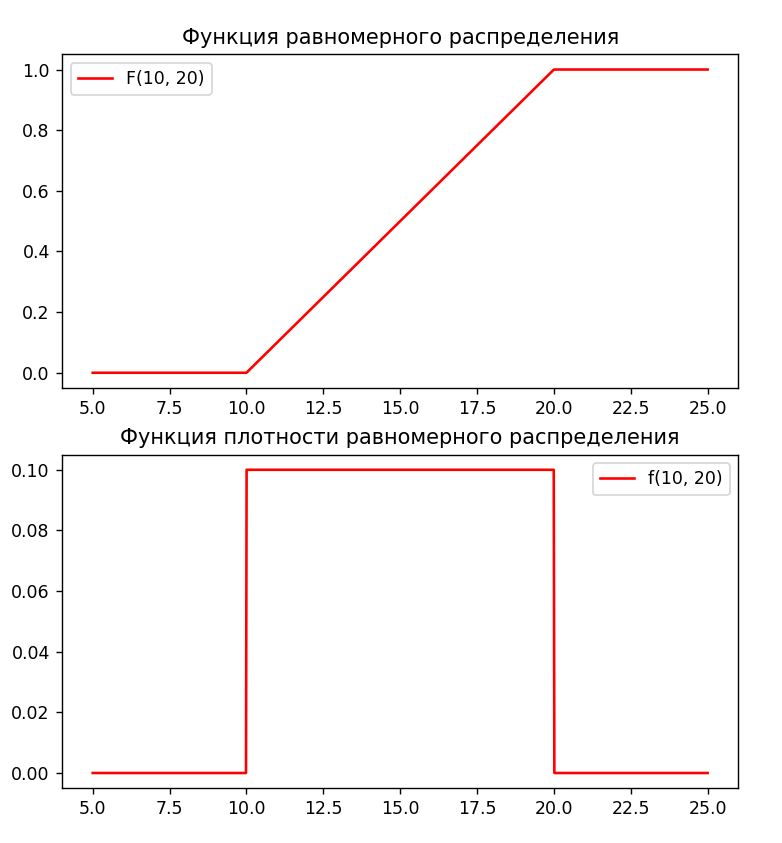
\includegraphics[scale=0.6]{1}
        		\caption{График зависимости температуры $T(x)$  от координаты $x$ при заданных выше параметрах}
        		\label{fig:res1}
        	\end{center}
        \end{figure}
  \newpage
  \item График зависимости $T(x)$ при $F_0$ = -10 Вт/см2.
  
  \begin{figure}[H]
        	\begin{center}
        		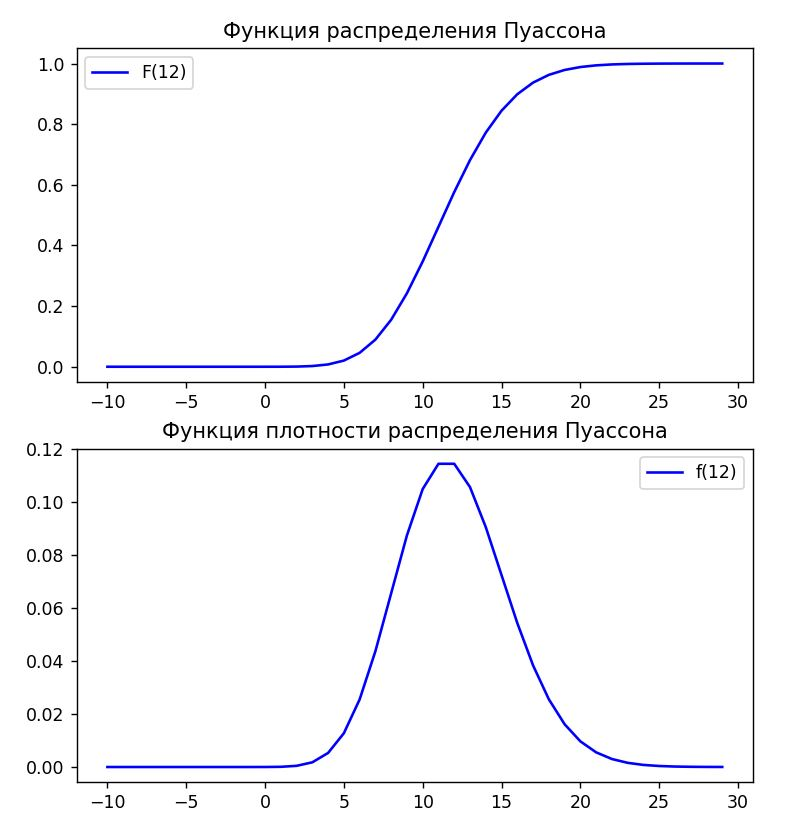
\includegraphics[scale=0.6]{2}
        		\caption{График зависимости $T(x)$ при $F_0$ = -10 Вт/см2}
        		\label{fig:res1}
        	\end{center}
        \end{figure}
        
  \item График зависимости $T(x)$ при увеличенных значениях $\alpha(x)$ (например, в 3 раза). 
  
  \begin{figure}[H]
        	\begin{center}
        		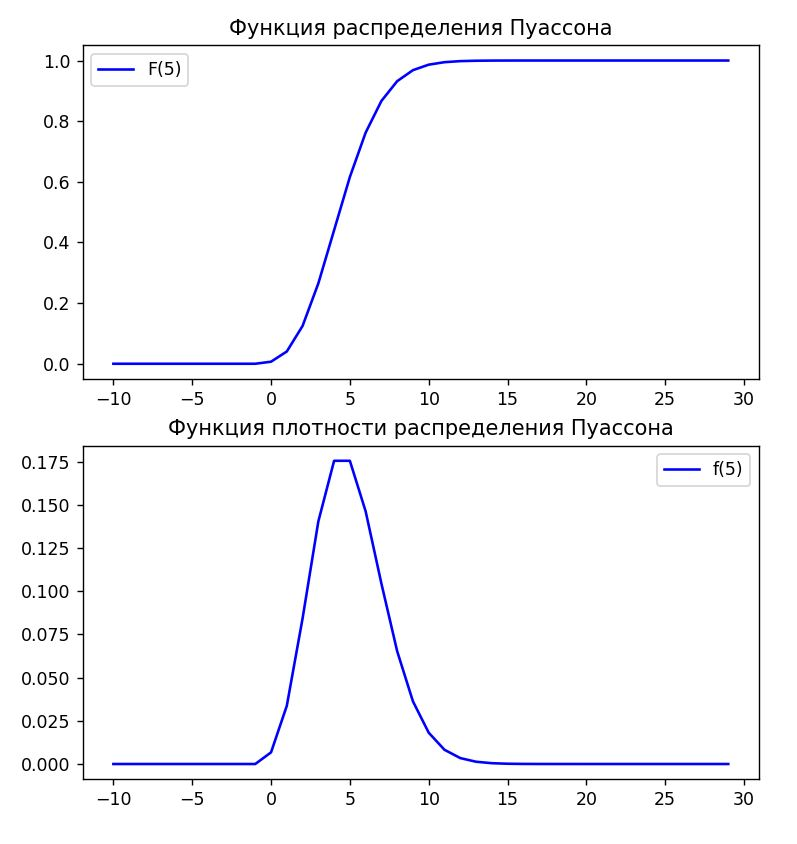
\includegraphics[scale=0.6]{3}
        		\caption{График зависимости $T(x)$ при увеличенных значениях $\alpha(x)$ (например, в 3 раза)}
        		\label{fig:res1}
        	\end{center}
        \end{figure}
        
   \item График зависимости $T(x)$ при $F_0$ = 0.
   
   \begin{figure}[H]
        	\begin{center}
        		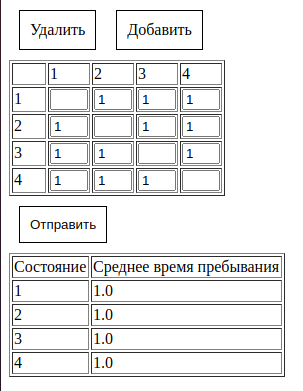
\includegraphics[scale=0.6]{4}
        		\caption{График зависимости $T(x)$ при $F_0$ = 0}
        		\label{fig:res1}
        	\end{center}
        \end{figure}
        
\end{enumerate}

\section{Ответы на вопросы}

\begin{enumerate}
  \item Какие способы тестирования программы можно предложить?\\
Увеличить коэффициент теплоотдачи ($\alpha_0, \alpha_N$). Стержень будет отдавать больше тепла, увеличится скорость понижения температуры.
\begin{figure}[H]
        	\begin{center}
        		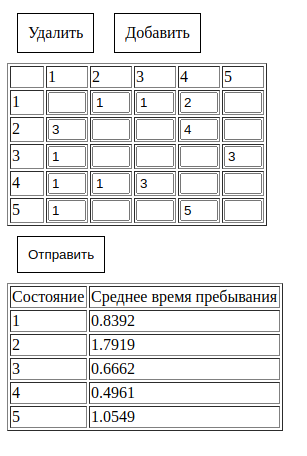
\includegraphics[scale=0.5]{5}
        		\caption{График зависимости $T(x)$ при $\alpha_0 = 0.5, \alpha_N = 0.1$}
        		\label{fig:res1}
        	\end{center}
        \end{figure}

  \item Получите  простейший разностный аналог нелинейного краевого условия при  $x = l$ $$-k(l)\frac{dT}{dx}=\alpha_N(T(l)-T_0)+\varphi(T),$$
где $\varphi(T)$ заданная функция.\\       

Построим разностную схему методом разностной апроксимации на равномерной сетке с шагом h. 

Аппроксимируем производную:

$$\frac{dT}{dx}=\frac{T(x)-T(x-h)}{h}$$

При $x=l$:

$$\frac{dT}{dx}=\frac{T_l-T_{l - 1}}{h}$$

Подставим в исходное уравнение:

$$-k_l\frac{T_{l}-T_{l-1}}{h}=\alpha_N(T_l-T_0)+\varphi(T_l)$$

$$-k_lT_{l}+k_lT_{l-1}=\alpha_NhT_l-\alpha_NhT_0+\varphi(T_l)h$$

$$-(k_l+\alpha_Nh)T_{l}+k_lT_{l-1}=\varphi(T_l)h-\alpha_NhT_0\eqno(23)$$ 

	\item Опишите алгоритм применения метода прогонки, если при  $x = 0$ краевое условие линейное (как в настоящей работе), а при $x = l$, как в п.2.\\

Для прямого хода при $x = 0$ начальные прогоночные коэффициенты $\varepsilon, \eta$ равны:
$$
\begin{aligned}
&\varepsilon_1=-\frac{M_0}{K_0}\\
&\eta_1=\frac{P_0}{K_0}
\end{aligned}
$$

Вычислим все прогоночные коэффициенты:
$$
\begin{aligned}
&\varepsilon_{n+1} = \frac{C_n}{B_n-A_n\varepsilon_n}\\
&\eta_{n+1} = \frac{D_n+A_n\eta_n}{B_n-A_n\varepsilon_n}
\end{aligned}
$$

Находим $y_N$ путем решения уравнения (23), полученного в п. 2, методом дихотомии. Обратным ходом найдем все коэффициенты до $y_0$.

Все значения неизвестных $y_n$ находятся по основной прогоночной формуле: 
$$ y_n=\varepsilon_{n+1}y_{n+1}+\eta_{n+1} $$

	\item Опишите алгоритм определения единственного значения сеточной функции $y_p$ в одной заданной точке $p$. Использовать встречную прогонку, т.е. комбинацию правой и левой прогонок (лекция №8). Краевые условия линейные.
	
Обозначим $i=p$, $0<p<N$. 

Правая прогонка.\\
Область: $0\le i \le p+1$\\
Прогоночные коэффициенты $\alpha_i, \beta_i$:

$$\alpha_{i+1}=\frac{C_i}{B_i-\alpha_iA_i}$$

$$\beta_{i+1}=\frac{A_i\beta_i+D_i}{C_i-\alpha_iA_i}$$

Левая прогонка.\\
Область: $p\le i \le N$ \\
Прогоночные коэффициенты $\varepsilon_i, \eta_i$:

$$\varepsilon_{i}=\frac{C_i}{B_i-\varepsilon_{i+1}A_i}$$

$$\eta_{i}=\frac{A_i\eta_{i+1}+D_i}{B_i-\varepsilon_{i+1}A_i}$$

Тогда при $i=p$:

$$y_p=\alpha_{p+1}y_{p+1}+\beta_{p+1},$$

$$y_{p+1}=\varepsilon_{p+1}y_{p}+\eta_{p+1},$$

$$y_{p}=\frac{\beta_{p+1}+\alpha_{p+1}\eta_{p+1}}{1-\alpha_{p+1}\varepsilon_{p+1}}$$

\end{enumerate}

\section*{Вывод}

В ходе лабораторной работы были получены навыки разработки  алгоритмов решения краевой задачи при реализации моделей, построенных на  ОДУ второго порядка.

\end{document}